\documentclass{article}
\title{Homework3.3}
\author{Blue}
\date{20230224}
\usepackage{geometry}
\geometry{a4paper,scale=0.8}
\usepackage{graphicx}
\usepackage{float}
\usepackage{indentfirst}
\usepackage[namelimits]{amsmath} %数学公式
\usepackage{amssymb}             %数学公式
\usepackage{color}
\usepackage{longtable}
\usepackage{listings}
\lstset{
language=Matlab,
numbers=left,
keywordstyle=\color{blue},
numberstyle=\tiny,
breaklines=true,
extendedchars=flase
}
\begin{document}
\maketitle
\section{Circular Orbit}

Using the initial condition, we get the circular orbit. Although it's not a perfect circle, it looks close to it. Also, we have the energy of the planet. It has accuracy to 9 decimal places.
\begin{figure}[htbp]
    \centering
    \begin{minipage}{0.45\linewidth}
        \centering
        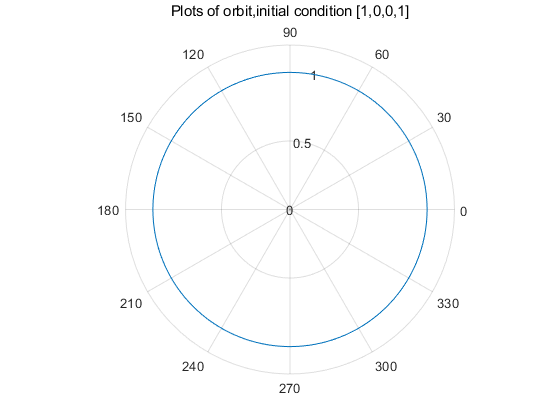
\includegraphics[width=\linewidth]{ar1.png}
        \caption{The circular orbit}
        \label{fig:picture1}
    \end{minipage}
    \hfill
    \begin{minipage}{0.45\linewidth}
        \centering
        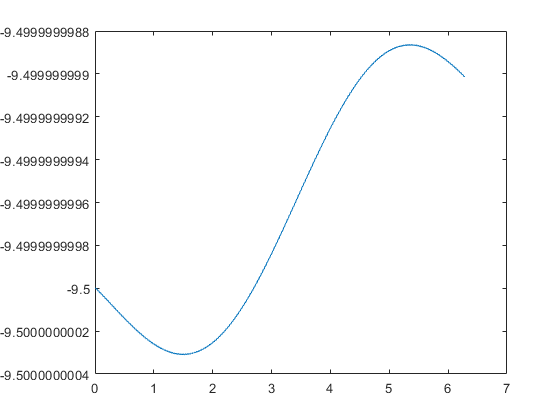
\includegraphics[width=\linewidth]{ar11.png}
        \caption{The energy of circular orbit planet}
        \label{fig:picture2}
    \end{minipage}
\end{figure}

If we change the initial condition. We can get a ellipse orbit. The energy of the ellipse orbit planet changes periodically.
\begin{figure}[htbp]
    \centering
    \begin{minipage}{0.45\linewidth}
        \centering
        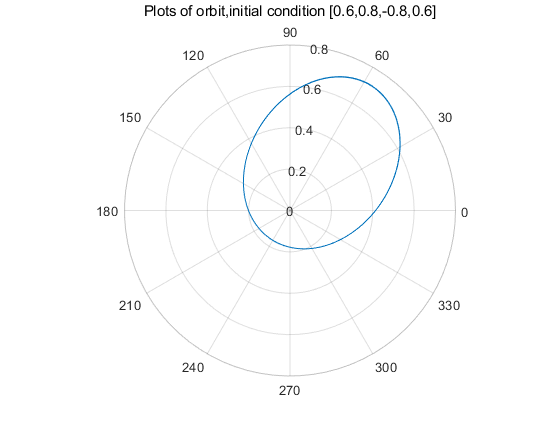
\includegraphics[width=\linewidth]{ar2.png}
        \caption{The Elliptical Orbit}
    \end{minipage}
    \hfill
    \begin{minipage}{0.45\linewidth}
        \centering
        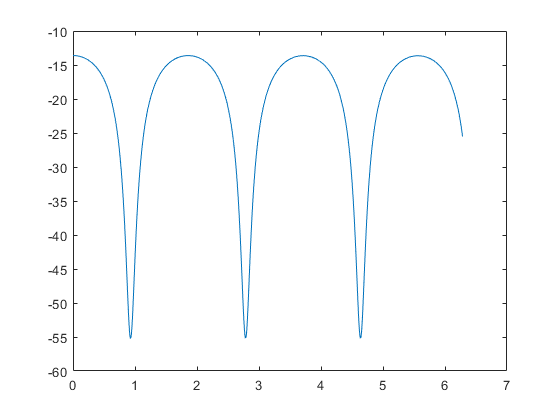
\includegraphics[width=\linewidth]{ar21.png}
        \caption{The energy of Elliptical Orbit planet}
    \end{minipage}
\end{figure}
\clearpage



\section{Elliptical Orbit}
First we use forward Euler's method, it's not a good method as shown below. The orbit and the energy changes as the time grows. We set the initial condition as $r=[0.36,0.64],v=[-0.48,0.48]$.
\begin{figure}[htbp]
    \centering
    \begin{minipage}{0.45\linewidth}
        \centering
        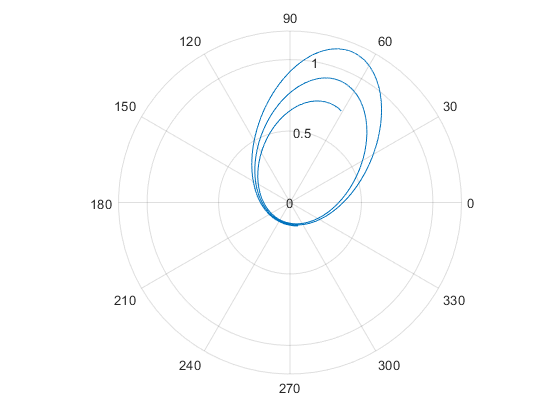
\includegraphics[width=0.8\linewidth]{br1.png}
        \caption{The Elliptical Orbit using forward Euler's method.}
    \end{minipage}
    \hfill
    \begin{minipage}{0.45\linewidth}
        \centering
        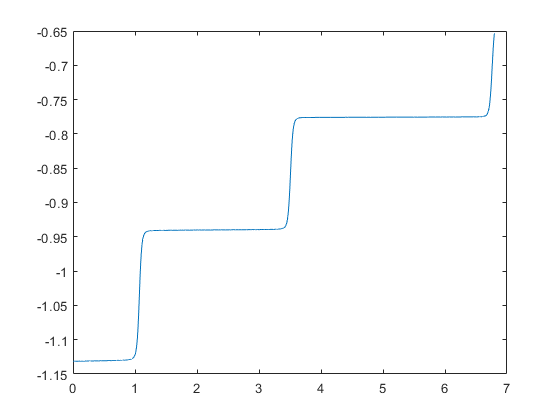
\includegraphics[width=0.8\linewidth]{br11.png}
        \caption{The energy of Elliptical Orbit planet}
    \end{minipage}
\end{figure}

Then we try Verlet's method, whose accuracy is much better than Euler's method.
\begin{figure}[htbp]
    \centering
    \begin{minipage}{0.45\linewidth}
        \centering
        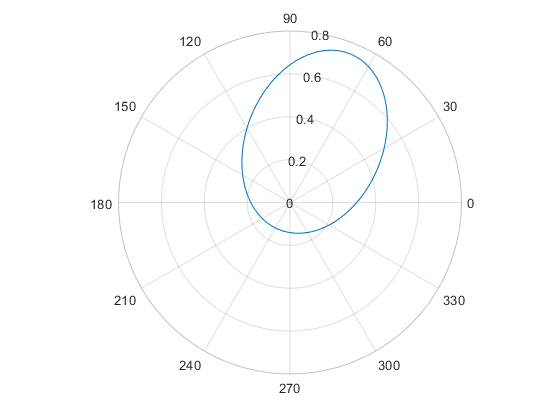
\includegraphics[width=0.8\linewidth]{br2.png}
        \caption{The Elliptical Orbit using Verlet's method}
    \end{minipage}
    \hfill
    \begin{minipage}{0.45\linewidth}
        \centering
        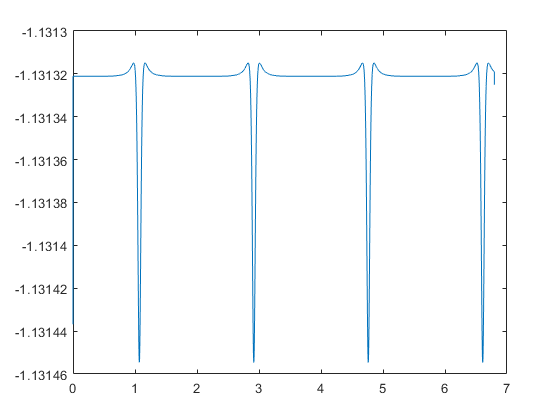
\includegraphics[width=0.8\linewidth]{br21.png}
        \caption{The energy of Elliptical Orbit planet}
    \end{minipage}
\end{figure}

Finally, we try 0de45 which is the most accurate one.
\begin{figure}[htbp]
    \centering
    \begin{minipage}{0.45\linewidth}
        \centering
        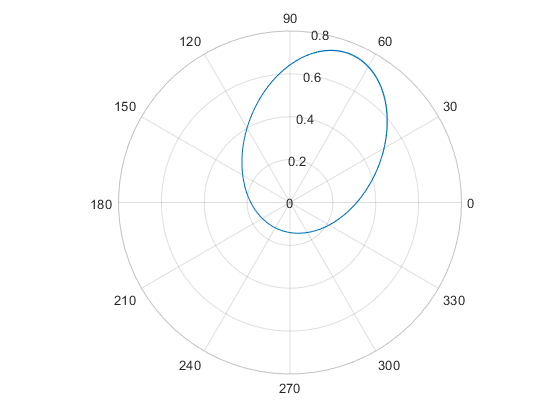
\includegraphics[width=0.8\linewidth]{br3.png}
        \caption{The Elliptical Orbit using ode45}
    \end{minipage}
    \hfill
    \begin{minipage}{0.45\linewidth}
        \centering
        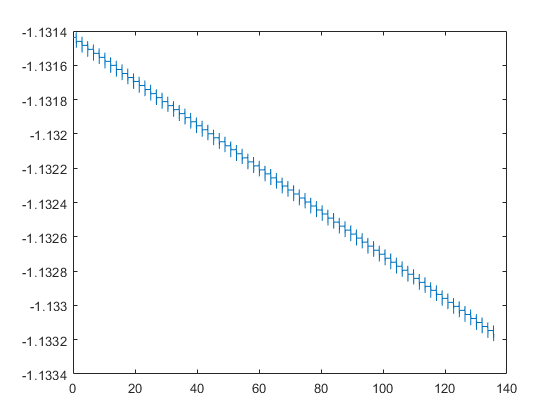
\includegraphics[width=0.8\linewidth]{br31.png}
        \caption{The energy of Elliptical Orbit planet}
    \end{minipage}
\end{figure}
\clearpage
If we set the initial speed larger than 1. We get a bad result, showing that the planet is escaping. We choose condition as $r=[0.72,1.2],v=[-0.96,0.9]$. Even the most accurate one ode45 shows that it will escape. The other two methods shows similarly.
\begin{figure}[htbp]
    \centering
    \begin{minipage}{0.45\linewidth}
        \centering
        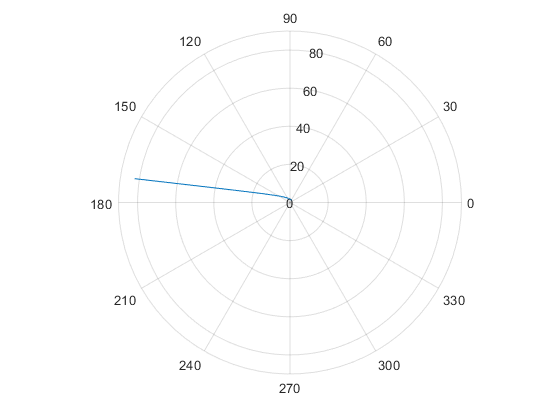
\includegraphics[width=0.8\linewidth]{br4.png}
        \caption{The Escaping planet using ode45}
    \end{minipage}
    \hfill
    \begin{minipage}{0.45\linewidth}
        \centering
        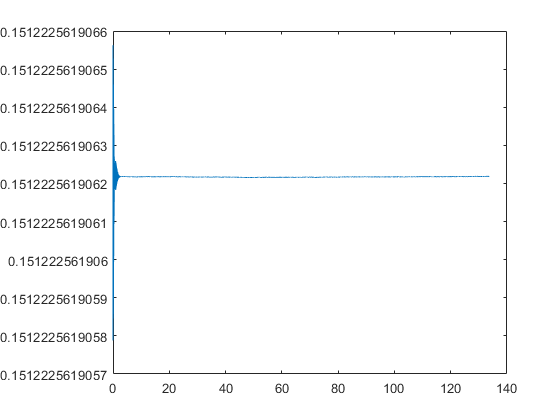
\includegraphics[width=0.8\linewidth]{br41.png}
        \caption{The energy of Escaping planet}
    \end{minipage}
\end{figure}

If I need to choose between three methods, I will choose 0de45 since its a function built in MATLAB. Also it should be the most accurate one.


\section{Multiple planets \& Movies}
I produce two movies. One is elliptical orbit, another is cicular orbit. I choose initial condition carefully. The scripts are attached to the end of the document.


\section{code}
\subsection{Circular Orbit}
\begin{lstlisting}
G=1;
m0=10;
n0=2;
t0=2*pi;
r0=[1,0,0,1];
r1=[0.4,0.6,-0.6,0.4];
opt1=odeset('MaxStep',t0/200);
[T1,R1]=ode45(@(t,r) myode(t,r,n0),[0 t0],r0,opt1);
[T2,R2]=ode45(@(t,r) myode(t,r,n0),[0 t0],r1,opt1);
[theta1,rho1]=cart2pol(R1(:,1),R1(:,2));
figure(1)
polarplot(theta1,rho1);
[theta2,rho2]=cart2pol(R2(:,1),R2(:,2));
title('Plots of orbit,initial condition [1,0,0,1]');
figure(2)
polarplot(theta2,rho2);
title('Plots of orbit,initial condition [0.6,0.8,-0.8,0.6]');
figure(3)
E=zeros(size(T1));
[m,n]=size(T1);
for i=1:m
    E(i,:)=-G*m0/norm(R1(i,1:2))+(norm(R1(i,3:4))^2)/2;
end
plot(T1,E)
figure(4)
E=zeros(size(T2));
[m,n]=size(T2);
for i=1:m
    E(i,:)=-G*m0/norm(R2(i,1:2))+(norm(R2(i,3:4))^2)/2;
end
plot(T2,E)
function drdt=myode(t,r,n)%in r and drdt 1-n is the original function,n+1-2n is dirivative
G=1;
m0=1.0;
drdt=zeros(2*n,1);
r2=norm(r(1:n));
for i=1:n
    drdt(i)=r(n+i);
    drdt(n+i)=-G*m0*r(i)/(r2^3);
end
end
\end{lstlisting}



\subsection{Elliptical Orbit}
\begin{lstlisting}
G=1;
m0=1;
n0=2;
N=10000;
%r and v are row vector each one
r=zeros(N+1,n0);
v=zeros(N+1,n0);
a=0.6;
b=0.8;
cos1=0.6;
sin1=0.8;
% a=1;
% b=1;
% cos1=sqrt(2)/2;
% sin1=sqrt(2)/2;
r(1,:)=[a*cos1,b*sin1];
v(1,:)=[-a*sin1,b*cos1];
T=2*pi*norm(r(1,:))/norm(v(1,:));
dt=T/N;
for i=2:N+1
    r(i,:)=r(i-1,:)+dt*v(i-1,:);
    v(i,:)=v(i-1,:)+dt*(-G*m0*r(i-1,:)/(norm(r(i-1,:)))^3);
end
figure(1)
[theta1,rho1]=cart2pol(r(:,1),r(:,2));
polarplot(theta1,rho1);
figure(2)
t1=linspace(0,T,N+1);
E=zeros(N+1,1);
for i=1:N+1
    E(i,:)=-G*m0/norm(r(i,:))+(norm(v(i,:))^2)/2;
end
plot(t1,E);

%Verlet's method 
r1=zeros(N+1,n0);
v1=zeros(N+1,n0);
r1(1:2,:)=r(1:2,:);
v1(1:2,:)=v(1:2,:);
for i=3:N+1
   r1(i,:)=2*r1(i-1,:)-r1(i-2,:)+dt^2*(-G*m0*r1(i-1,:)/(norm(r1(i-1,:)))^3);
   v1(i-1,:)=(r1(i,:)-r1(i-2,:))/(2*dt);
end
v1(N+1,:)=v1(N,:)+dt*(-G*m0*r1(N,:)/(norm(r1(N,:)))^3);
figure(3)
[theta2,rho2]=cart2pol(r1(:,1),r1(:,2));
polarplot(theta2,rho2);
figure(4)
t2=linspace(0,T,N+1);
E1=zeros(N+1,1);
for i=1:N+1
    E1(i,:)=-G*m0/norm(r1(i,:))+(norm(v1(i,:))^2)/2;
end
plot(t2,E1);


%ode45
r0=[a*cos1,b*sin1,-a*sin1,b*cos1];
opt1=odeset('MaxStep',T/500);
[T1,R1]=ode45(@(tk,rk) myode(tk,rk,n0),[0 20*T],r0,opt1);
figure(5)
[theta3,rho3]=cart2pol(R1(:,1),R1(:,2));
polarplot(theta3,rho3);
figure(6)
t2=linspace(0,T,N+1);
E2=zeros(size(T1));
[m,n]=size(T1);
for i=1:m
    E2(i,:)=-G*m0/norm(R1(i,1:2))+(norm(R1(i,3:4))^2)/2;
end
plot(T1,E2)
function drdt=myode(t,r,n)%in r and drdt 1-n is the original function,n+1-2n is dirivative
G=1;
m0=1.0;
drdt=zeros(2*n,1);
r2=norm(r(1:n));
for i=1:n
    drdt(i)=r(n+i);
    drdt(n+i)=-G*m0*r(i)/(r2^3);
end
end
\end{lstlisting}


\subsection{Multiple planets and Movies}
\subsubsection{Elliptical Orbit}
\begin{lstlisting}
n0=2;
t0=8*pi;
a=0.8;
b=1.4;
cos1=0.6;
sin1=0.8;
r0=[0.4*a*cos1,0.4*b*sin1,-a*sin1/sqrt(0.4),b*cos1/sqrt(0.4)];
r1=[0.45*a*cos1,0.45*b*sin1,-a*sin1/sqrt(0.45),b*cos1/sqrt(0.45)];
r2=[0.6*a*cos1,0.6*b*sin1,-a*sin1/sqrt(0.6),b*cos1/sqrt(0.6)];
r3=[0.8*a*cos1,0.8*b*sin1,-a*sin1/sqrt(0.8),b*cos1/sqrt(0.8)];
r4=[a*cos1,b*sin1,-a*sin1,b*cos1];
opt1=odeset('MaxStep',2*pi/50);
sol0=ode45(@(t,r) myode(t,r,n0),[0 t0],r0,opt1);
sol1=ode45(@(t,r) myode(t,r,n0),[0 t0],r1,opt1);
sol2=ode45(@(t,r) myode(t,r,n0),[0 t0],r2,opt1);
sol3=ode45(@(t,r) myode(t,r,n0),[0 t0],r3,opt1);
sol4=ode45(@(t,r) myode(t,r,n0),[0 t0],r4,opt1);
Nt=400;
t=linspace(0,t0,Nt);
R0=deval(sol0,t);
R1=deval(sol1,t);
R2=deval(sol2,t);
R3=deval(sol3,t);
R4=deval(sol4,t);

vidobj = VideoWriter('movie1.mp4','mpeg-4');
open(vidobj);
for k=1:Nt
    scatter(0,0,50,'rd','markerfacecolor','r'); hold on;
    scatter(R0(1,k),R0(2,k),20,'ok','markerfacecolor','k');
    scatter(R1(1,k),R1(2,k),20,'ok','markerfacecolor','y');
    scatter(R2(1,k),R2(2,k),40,'ok','markerfacecolor','b');
    scatter(R3(1,k),R3(2,k),40,'ok','markerfacecolor','r');
    scatter(R4(1,k),R4(2,k),80,'ok','markerfacecolor','m');
    plot(R0(1,1:80),R0(2,1:80));
    plot(R1(1,:),R1(2,:));
    plot(R2(1,:),R2(2,:));
    plot(R3(1,:),R3(2,:));
    plot(R4(1,:),R4(2,:));
    xlim([-3 1]);
    ylim([-1.3 2.1]);
    pbaspect([100 100 1])
    set(gca,'FontSize',20);
    set(gcf,'color','w');
    box on;
    title('My solar system');
    currFrame = getframe(gcf);
    hold off;
    writeVideo(vidobj,currFrame);
end
close(vidobj);


function drdt=myode(t,r,n)%in r and drdt 1-n is the original function,n+1-2n is dirivative
G=1;
m0=1.0;
drdt=zeros(2*n,1);
r2=norm(r(1:n));
for i=1:n
    drdt(i)=r(n+i);
    drdt(n+i)=-G*m0*r(i)/(r2^3);
end
end
\end{lstlisting}

\subsubsection{Circular Orbit}
\begin{lstlisting}
n0=2;
t0=2*pi;
r0=[0.2,0,0,sqrt(1/0.2)];
r1=[0.4,0,0,sqrt(1/0.4)];
r2=[0.6,0,0,sqrt(1/0.6)];
r3=[0.8,0,0,sqrt(1/0.8)];
r4=[1,0,0,1];
opt1=odeset('MaxStep',2*pi/50);
sol0=ode45(@(t,r) myode(t,r,n0),[0 t0],r0,opt1);
sol1=ode45(@(t,r) myode(t,r,n0),[0 t0],r1,opt1);
sol2=ode45(@(t,r) myode(t,r,n0),[0 t0],r2,opt1);
sol3=ode45(@(t,r) myode(t,r,n0),[0 t0],r3,opt1);
sol4=ode45(@(t,r) myode(t,r,n0),[0 t0],r4,opt1);
Nt=300;
t=linspace(0,t0,Nt);
R0=deval(sol0,t);
R1=deval(sol1,t);
R2=deval(sol2,t);
R3=deval(sol3,t);
R4=deval(sol4,t);

vidobj = VideoWriter('movie.mp4','mpeg-4');
open(vidobj);
for k=1:Nt
    scatter(0,0,100,'rd','markerfacecolor','r'); hold on;
    scatter(R0(1,k),R0(2,k),20,'ok','markerfacecolor','k');
    scatter(R1(1,k),R1(2,k),20,'ok','markerfacecolor','y');
    scatter(R2(1,k),R2(2,k),40,'ok','markerfacecolor','b');
    scatter(R3(1,k),R3(2,k),40,'ok','markerfacecolor','r');
    scatter(R4(1,k),R4(2,k),80,'ok','markerfacecolor','m');
    plot(R0(1,1:80),R0(2,1:80));
    plot(R1(1,:),R1(2,:));
    plot(R2(1,:),R2(2,:));
    plot(R3(1,:),R3(2,:));
    plot(R4(1,:),R4(2,:));
    xlim([-1 1])
    ylim([-1 1])
    pbaspect([100 100 1])
    set(gca,'FontSize',20);
    set(gcf,'color','w');
    box on;
    title('My solar system');
    currFrame = getframe(gcf);
    hold off;
    writeVideo(vidobj,currFrame);
end
close(vidobj);

function drdt=myode(t,r,n)%in r and drdt 1-n is the original function,n+1-2n is dirivative
G=1;
m0=1.0;
drdt=zeros(2*n,1);
r2=norm(r(1:n));
for i=1:n
    drdt(i)=r(n+i);
    drdt(n+i)=-G*m0*r(i)/(r2^3);
end
end
\end{lstlisting}





\end{document}